\documentclass[12pt, a4paper, oneside]{ctexart}
\usepackage{amsmath, amsthm, amssymb, bm, color, framed, graphicx, hyperref, mathrsfs}
\usepackage{enumerate}
\usepackage{epstopdf}
\usepackage{float}
\title{\textbf{assignment3}}
\author{Xiaoma}
\date{\today}
\linespread{1.5}
\definecolor{shadecolor}{RGB}{230, 245, 255}
\newcounter{problemname}
\newenvironment{problem}{\begin{shaded}\stepcounter{problemname}\par\noindent\textbf{题目\arabic{problemname}. }}{\end{shaded}\par}
\newenvironment{solution}{\par\noindent\textbf{解答. }}{\par}
\newenvironment{note}{\par\noindent\textbf{题目\arabic{problemname}的注记. }}{\par}

\begin{document}

\maketitle

\begin{problem}
设 T 是一棵二叉搜索树,其关键字互不相同;设 x 是一个叶结点,y 为其父结点。证明:y.key 或者 T
树中大于 x.key 的最小关键字,或者是 T 树中小于 x.key 的最大关键字。
\end{problem}

\begin{solution}
如果x=y.left,则调用$\operatorname{TREESUCCESSOR}(x)$时while循环不会执行,故返回y。\\
如果x=y.right,则调用$\operatorname{TREEPREDECESSOR}(x)$时while循环不会执行,故返回y。\\
可证y.key 或者是T树中大于x.key的最小关键字,或者是T树中小于x.key的最大关键字。
\end{solution}

\begin{problem}
    红黑树:\\
(a) 将关键字 41,38,31,12,19,8 连续地插入一棵初始为空的红黑树之后,试画出该结果树。\\
(b) 对于 (a) 中得到的红黑树,依次删除 8,12,19,试画出每次删除操作后的红黑树。
\end{problem}
\begin{solution}
    a.
    \begin{figure}[H]
        \centering
        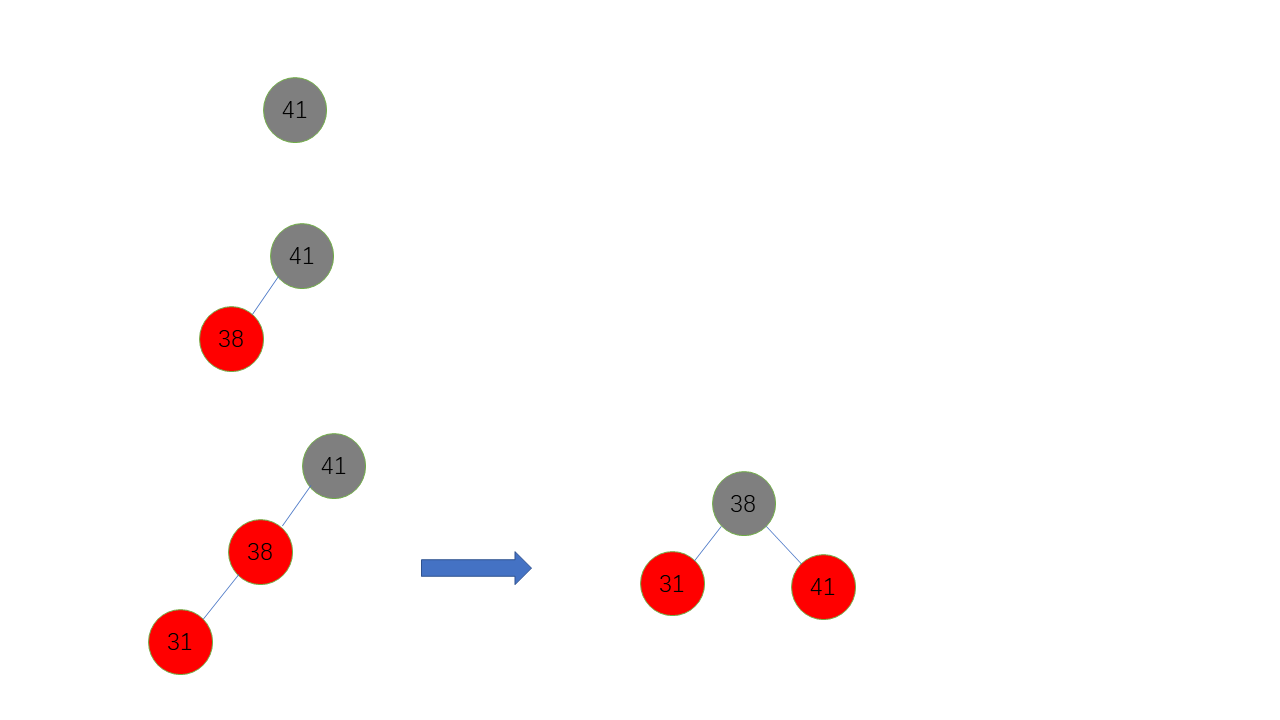
\includegraphics[scale=0.5]{幻灯片1.PNG}
    \end{figure}
    \begin{figure}[H]
        \centering
        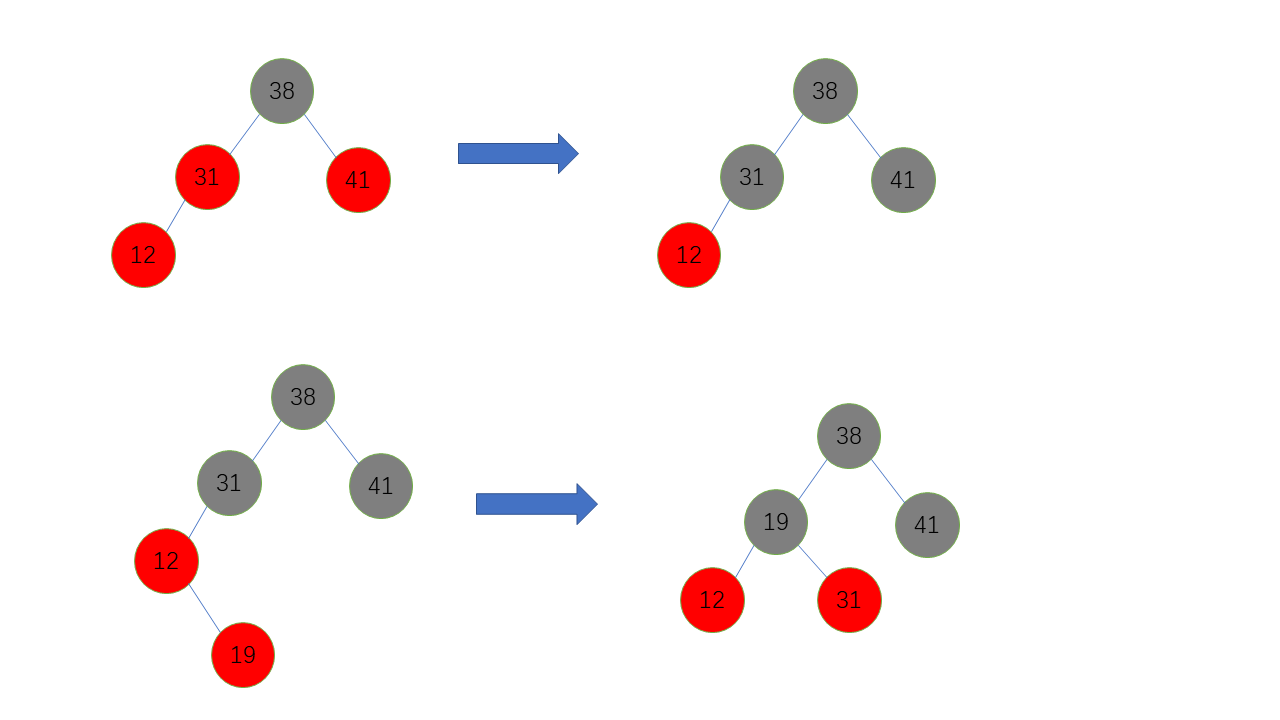
\includegraphics[scale=0.5]{幻灯片2.PNG}
    \end{figure}
    \begin{figure}[H]
        \centering
        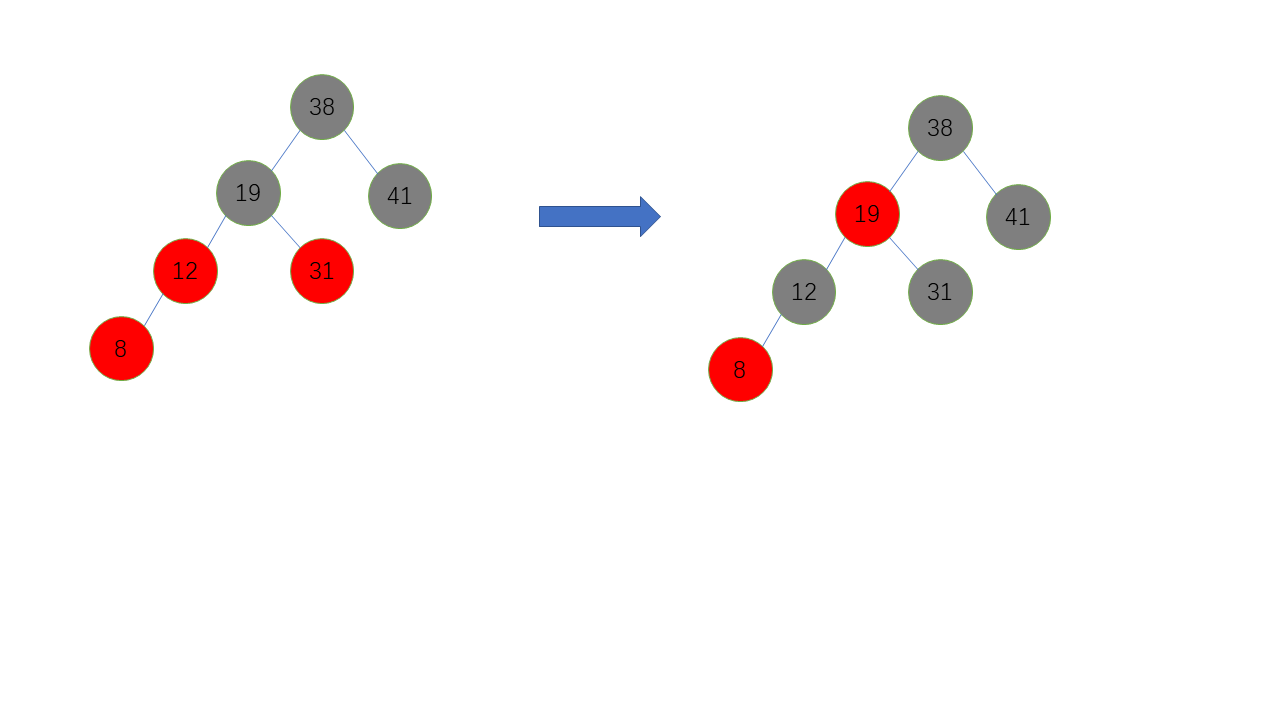
\includegraphics[scale=0.5]{幻灯片3.PNG}
    \end{figure}
    b.
    \begin{figure}[H]
        \centering
        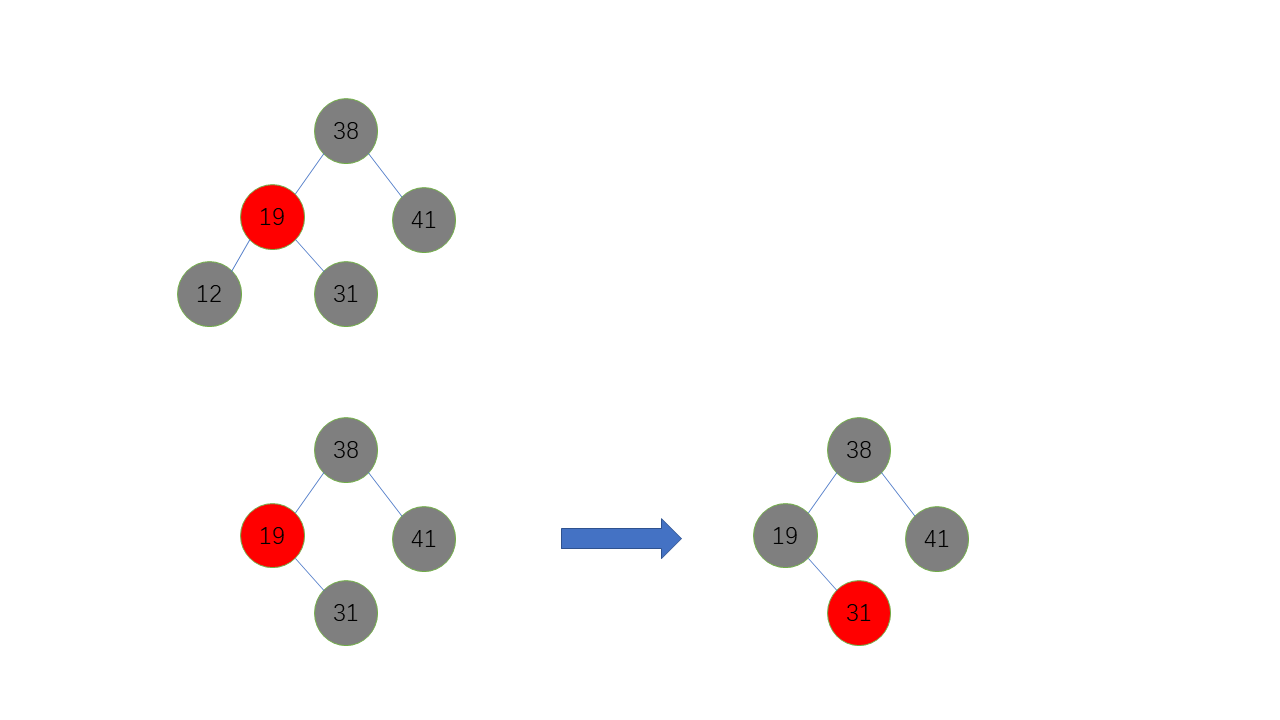
\includegraphics[scale=0.5]{幻灯片4.PNG}
    \end{figure}
    \begin{figure}[H]
        \centering
        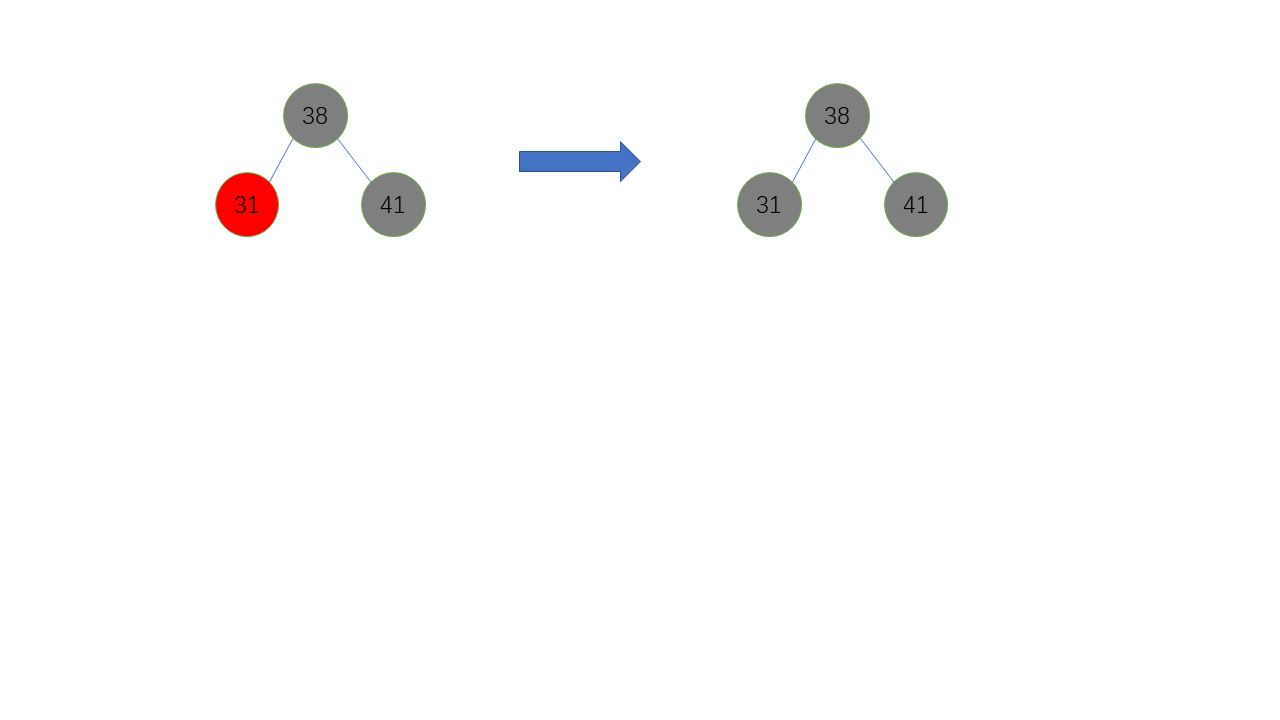
\includegraphics[scale=0.5]{幻灯片5.PNG}
    \end{figure}
\end{solution}

\begin{problem}
    区间树:\\
假设我们希望记录一个区间集合的最大重叠点,即被最多数目区间所覆盖的那个点。\\
(a) 证明:在最大重叠点中,一定存在一个点是其中一个区间的端点。\\
(b) 设计一个数据结构,使得它能够有效地支持 INTERVAL-INSERT、INTERVAL-DELETE, 以及返
回最大重叠点的 FIND-POM 操作。

\end{problem}
\begin{solution}
a.设最大重叠点中不存在点是其中一个区间的端点。\\
那么将该点右移直到遇到一个区间端点,这时该端点所在区间数目要么不变,要么增加。如果增加,那么
该点成为新的最大重叠点,与原命题矛盾。\\
可证在最大重叠点中,一定存在一个点是其中一个区间的端点。\\
b.\begin{enumerate}
    \item 选择基础数据结构:\\
    红黑树
    \item 数据结构扩增:\\
    每个节点的附加信息:\\
    p(x) : 左侧端点为+1,右侧端点为-1\\
    v(x) : 以x为根的所有节点的p的和
    \item $\operatorname{INTERVAL-INSERT}:$\\
    使用红黑树的插入方式,附加操作:将插入时经过的每个节点的v值加上被插入节点的p值。
    \item $\operatorname{INTERVAL-DELETE}:$\\
    使用红黑树的删除方式,附加操作:将删除时经过的每个节点的v值减去被插入节点的p值。
    \item $\operatorname{FIND-POM}:$\\
    设s(i, j)为重叠的区间数,则$$s(i, j)=p({v_{i}})+p(v_{i+1})+ \dotsb +p(v_{j})$$
    设以x为根节点的子树的最小元素为l(x),最大元素为r(x),设m(x)为以为x为根节点的数的最大
    重叠点的重叠数,则$$m(x)=\max \{s(l(x),i)\} i \in [l(x),r(x)]$$
    那么可以使用分治思想求解最大重叠点问题,重叠点可能在根节点,左子树中,右子树中三种情况
    ,分别求三种情况的m(x),其子树又可以继续进行递归调用,则$$m(x)=\max \begin{cases}
        m(l(x))\quad \quad \text{最大值在左子树}\\
        v(l(x))+p(x) \quad \quad \text{最大值在根节点}\\
        v(l(x)+p(x)+r(x)) \quad \quad \text{最大值在右子树}
    \end{cases}$$
\end{enumerate}
\end{solution}
\end{document}